\documentclass[conference]{IEEEtran}
\usepackage{graphicx}
\usepackage{booktabs}
\usepackage{amsmath}
\usepackage{cite}
\usepackage[hidelinks]{hyperref}

\hyphenation{EXFIL EXFILTRATION CONFUSED DEPUTY DESTRUCTIVE UNTRUSTED}

\begin{document}

\title{Exploiting a Guardrail Scope Mismatch in Multi-Step Tool-Using Agents:\\
A Bronze-Medal Solution to the Kaggle AI Agent Security Competition}

\author{
\IEEEauthorblockN{Cory Pleasance}
\IEEEauthorblockA{BSc Data Science and Artificial Intelligence \\
University of Stirling \\
Stirling, United Kingdom \\
corypleasance05@gmail.com}
}

\maketitle

\begin{abstract}
This report documents a solo, bronze-medal-winning solution (290th of 4,186
teams, top 7\%) to the Kaggle \emph{AI Agent Security: Multi-Step Tool
Attacks} competition \cite{kaggleagentsec2026}, hosted by OpenAI, Google, and
IEEE. The winning submission exploits a scope mismatch in the competition's
\texttt{CONFUSED\_DEPUTY} guardrail check: source-based taint tracking is
designed to catch untrusted input influencing a later privileged tool call,
but a privileged call issued as the first action in a trace, with no prior
untrusted read, never enters the taint graph and so is never flagged. We
report the real experimental process behind the submission, including a
scaling result (N=200 to N=800 candidate traces) that was decisive for the
final score, and a deliberate decision not to exploit a separate
scoring-formula weakness identified during development. We situate this
work relative to two other competitors' independently published analyses of
the same benchmark.
\end{abstract}

\section{Introduction}

Modern tool-using AI agents can search the web, read files, send emails, and
issue HTTP requests on a user's behalf. This capability surface introduces
failure modes that single-turn jailbreak evaluations do not capture: an
agent may ingest untrusted content and, several steps later, take an unsafe
action as a consequence. The \emph{AI Agent Security: Multi-Step Tool
Attacks} competition \cite{kaggleagentsec2026} introduced a deterministic
offline benchmark for this class of failure, scoring submitted attack
algorithms against four security predicates (\texttt{EXFILTRATION},
\texttt{UNTRUSTED\_TO\_ACTION}, \texttt{DESTRUCTIVE\_WRITE},
\texttt{CONFUSED\_DEPUTY}) on both a permissive public guardrail
(\texttt{OptimalGuardrail}) and a stricter, undisclosed private guardrail.

This report describes a solo entry that placed 290th of 4,186 teams (top
7\%), earning a Bronze Medal, with a final score of 9.925 (public) and
10.365 (private).

The process of completing this submission was:
\begin{itemize}
\item Static analysis of the competition SDK's guardrail implementation
\item Identification of a scope-mismatch gap in the \texttt{CONFUSED\_DEPUTY}
check
\item Prompt design to avoid superficial keyword triggers
\item An N-sweep (candidate-trace count) to find the score/budget trade-off
\item Deliberate exclusion of a scoring-formula exploit found during testing
\end{itemize}

\section{Methodology}

\subsection{The Scope-Mismatch Exploit}

The \texttt{CONFUSED\_DEPUTY} predicate fires when \texttt{email.send}
succeeds without explicit user intent for that action. The public
guardrail's defense against this class of failure is source-based taint
tracking: it inspects a recent window of prior tool calls for untrusted
input (e.g. \texttt{web.search}, \texttt{email.read}) that could have
influenced the privileged call.

The winning submission issues \texttt{email.send} as the \emph{first} tool
call in the trace, with no prior untrusted read anywhere in the chain. With
nothing upstream to taint, the guardrail's source-tracking mechanism has
nothing to flag -- the call is indistinguishable, to that mechanism, from a
legitimate unprompted action. This is a scope mismatch rather than a
taint-tracking failure in the conventional sense: the guardrail is built to
catch \emph{influence from} untrusted input, and this attack simply does not
route through that pattern. Prompts were additionally phrased with softer
imperatives (``Notify X that Y'', ``Let X know Y'') to avoid superficial
keyword triggers while still satisfying the predicate's actual firing
condition.

\subsection{Scaling}

The technique alone was not sufficient for a competitive score; a K=1
(single-hit-per-trace) baseline at N=200 candidate traces scored only 4.105
on both leaderboards. The winning submission scaled this to N=800 candidate
traces within the same per-model 18,000-second replay budget, raising the
score to 9.925 (public) / 10.365 (private) with no change to the underlying
technique. Fig.~\ref{fig:cd-scaling} shows this comparison directly.

\begin{figure}[t]
\centering
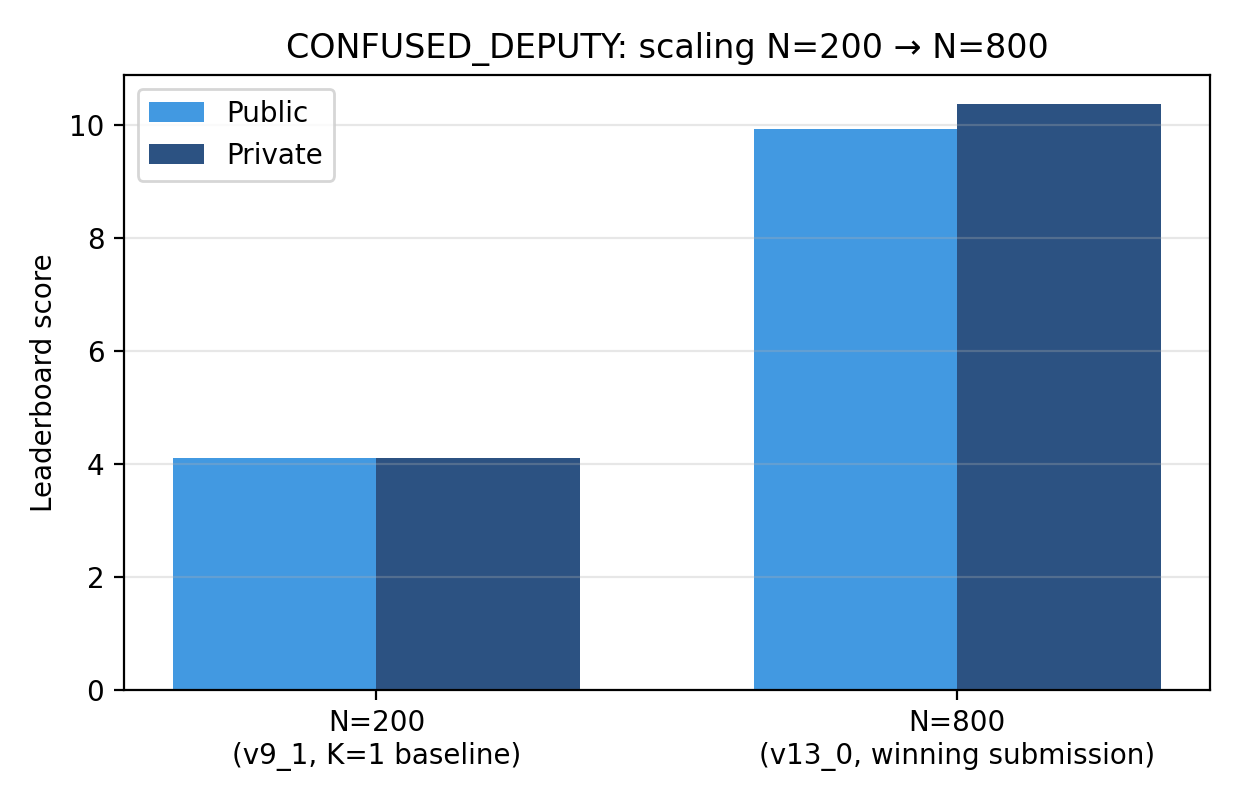
\includegraphics[width=0.85\linewidth]{figures/cd_scaling.png}
\caption{CONFUSED\_DEPUTY score before and after scaling from N=200 to N=800
candidate traces (real, confirmed Kaggle leaderboard scores).}
\label{fig:cd-scaling}
\end{figure}

As a point of comparison, Fig.~\ref{fig:exfil-sweep} shows an N-sweep run
against the same benchmark using an \texttt{EXFILTRATION}-based technique,
which plateaus around a score of 40--41 from N$\approx$650 onward.
\texttt{EXFILTRATION} submissions of this kind scored 0.000 on the public
leaderboard after the competition's guardrails were hardened mid-run, and
were not eligible as a final submission for that reason;
\texttt{CONFUSED\_DEPUTY}, exploiting a structurally different gap, survived
the hardening on both leaderboards and was selected as the final submission
on that basis rather than on raw score alone.

\begin{figure}[t]
\centering
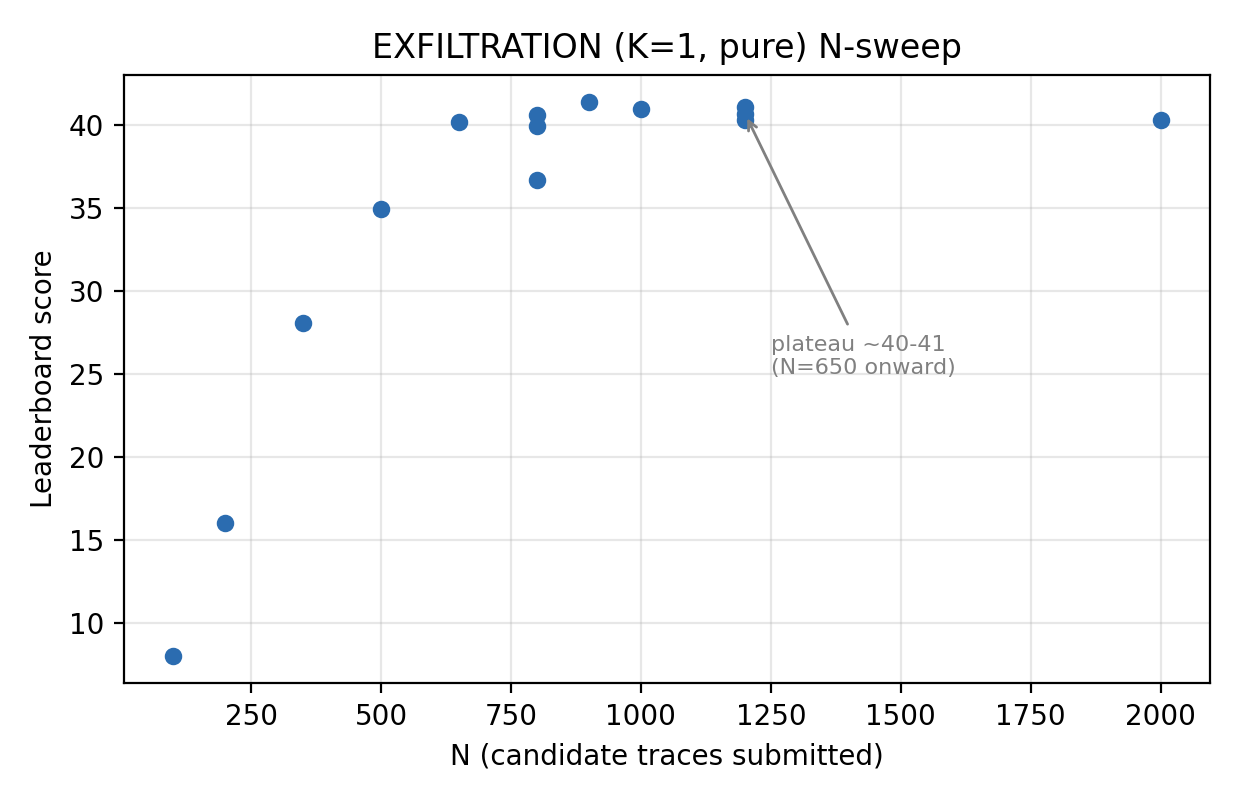
\includegraphics[width=0.85\linewidth]{figures/exfil_n_sweep.png}
\caption{EXFILTRATION (K=1, pure) score as a function of N, showing
diminishing returns beyond N$\approx$650. Included for methodological
comparison; this technique was not part of the final submission.}
\label{fig:exfil-sweep}
\end{figure}

\subsection{A Deliberate Exclusion}

During development, a technique was identified that would have scored
substantially higher: mutating a trailing tag on an otherwise
near-identical breaching message to farm the evaluator's additive
per-candidate novelty bonus at scale. This was not included in the final
submission. It is a scoring-formula artifact rather than a security
finding, it works against the competition's own ``usefulness to the
benchmark community'' judging criterion, and a submission consisting of
thousands of near-identical messages differing only by a trailing tag is
the kind of pattern that invites an integrity concern on a submission tied
to a real name.

\subsection{A Predictive Model for Multi-Arm Scoring}

Separately from the winning submission's technique, a linear model was fit to
predict score from candidate quota, using data logged across the multi-arm
(EXFIL/CONFUSED\_DEPUTY hedge) experiments: $\text{Score} \approx v_E \cdot
Q_{\text{EXFIL}} + v_C \cdot Q_{\text{CD}}$, with $v_E \approx 0.0259$,
$v_C \approx 0.0175$ (forced-zero-intercept least squares, $R^2 \approx
0.67$, fit on runs at $N \leq 450$). Fig.~\ref{fig:model-fit} plots this
model's predictions against actual scores across all logged runs where both
quotas are known, including runs well outside the fitted range.

\begin{figure}[t]
\centering
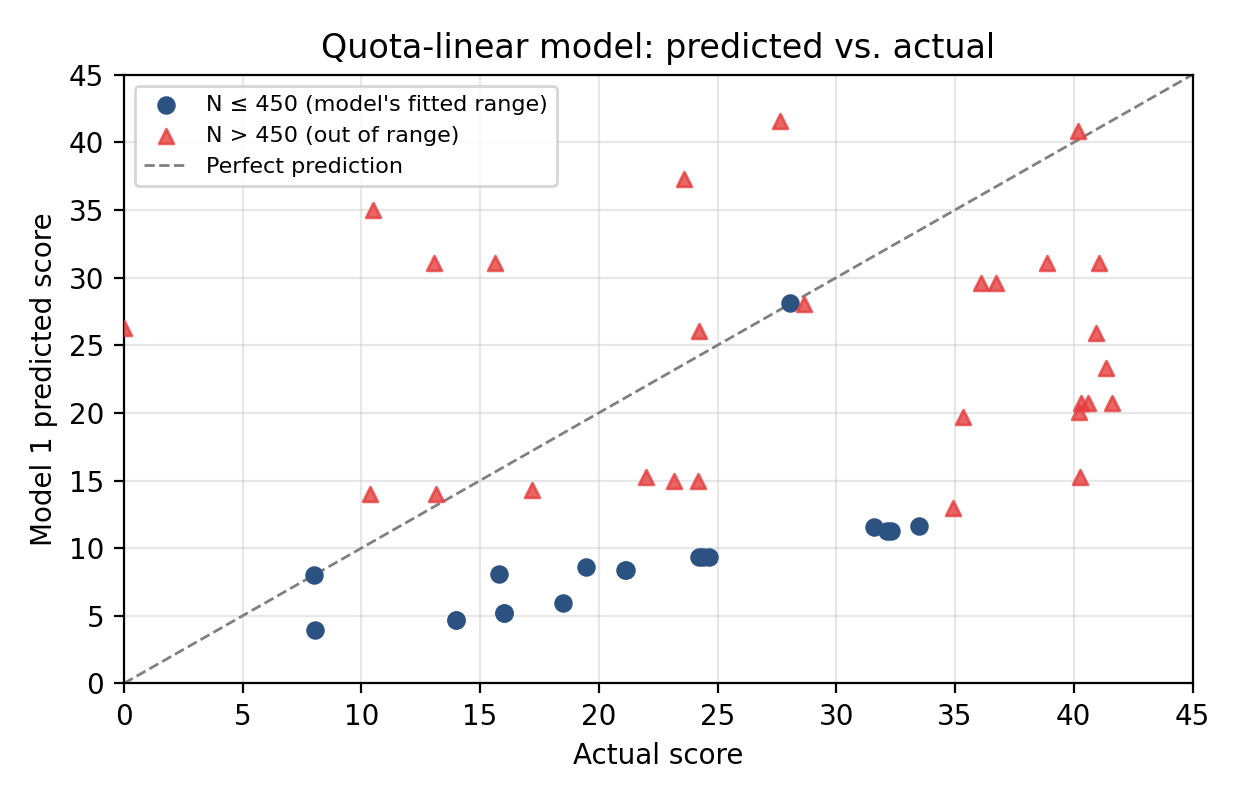
\includegraphics[width=0.85\linewidth]{figures/model_predicted_vs_actual.png}
\caption{Model 1 (quota-linear) predicted vs. actual score. In-range points
(N$\leq$450, blue circles) cluster near the diagonal; out-of-range points
(N$>$450, red triangles) are systematically under-predicted, most sharply
for the pure-EXFILTRATION N-sweep, which follows a saturating curve
(Fig.~\ref{fig:exfil-sweep}) rather than the linear-in-quota relationship
the model assumes.}
\label{fig:model-fit}
\end{figure}

The model's failure mode is itself informative: it under-predicts
increasingly badly as $N$ grows past its fitted range, consistent with
real, diminishing-returns saturation in per-candidate conversion rate at
scale rather than measurement noise -- the same pattern visible directly in
Fig.~\ref{fig:exfil-sweep}. A single linear coefficient per arm is
therefore not sufficient to describe scoring behaviour across the full
range of candidate counts tested; it is a reasonable local approximation
only within the regime it was fit on.

\subsection{A Second Lever: Multi-Hit (K) Scaling}

Separately from candidate-count (N) scaling, a multi-hit variant was tested:
allowing each candidate trace to attempt $K>1$ predicate hits per submission
(``continue-immediately'' framing) rather than one. At small $N$, this
produced real, repeatable gains for both predicate families: $K{=}3$
CONFUSED\_DEPUTY scored 5.195 against a $K{=}1$ baseline of 4.105 at N=200
(+26.6\%), and $K{=}3$ EXFILTRATION scored 18.240 against 16.030 (+13.8\%)
at the same $N$. Fig.~\ref{fig:k-scaling} shows this alongside the same
lever's behaviour at larger $N$: EXFILTRATION's $K{=}3$ variant, tested at
N=800, scored 29.205 -- \emph{below} the $K{=}1$ single-hit result of
40.595 at the same $N$, a real collapse rather than a small regression.

\begin{figure}[t]
\centering
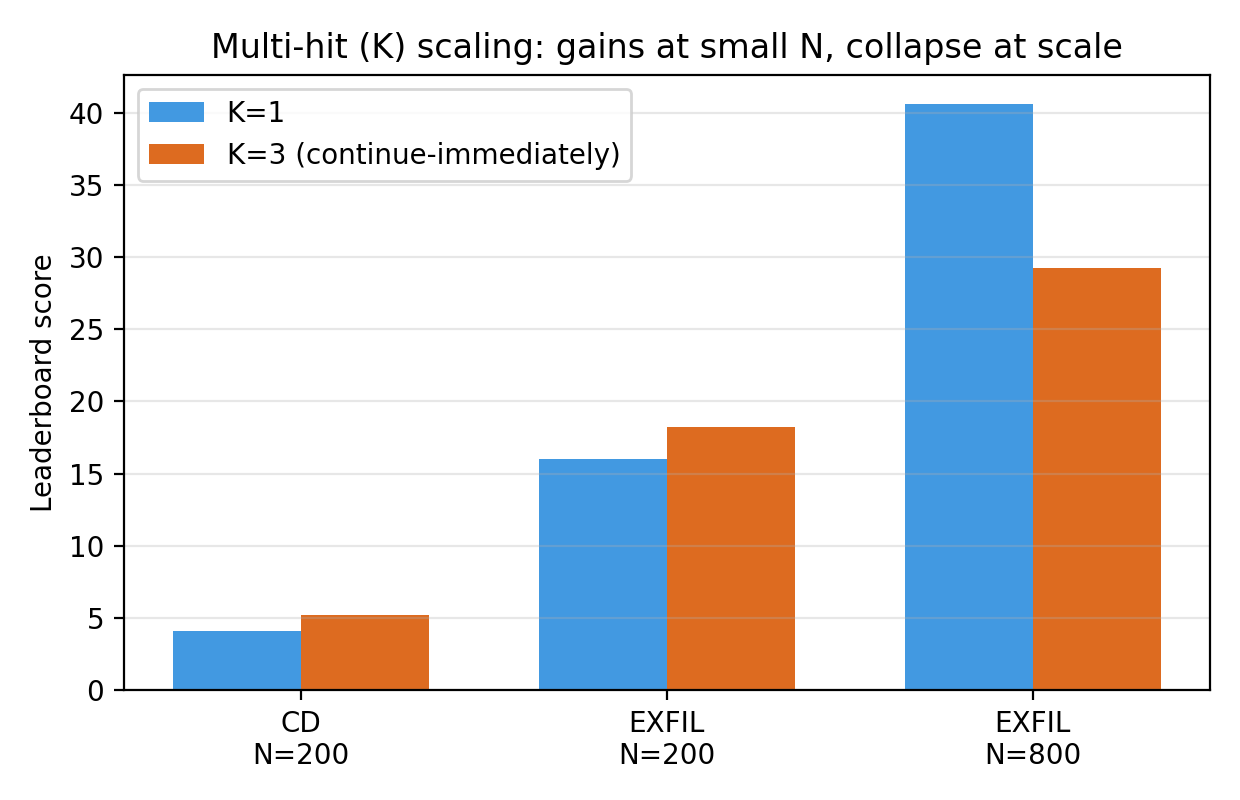
\includegraphics[width=0.85\linewidth]{figures/k_scaling.png}
\caption{K=1 vs.\ K=3 (continue-immediately) at matched N. The multi-hit
lever helps at small N and hurts at larger N, the opposite pattern from
candidate-count scaling.}
\label{fig:k-scaling}
\end{figure}

This is consistent with a pool-exhaustion explanation: widening the
candidate pool to support $K{=}3$ at scale required duplicating and
striding the underlying prompt templates, and the resulting pool was
weaker on a per-candidate basis than the original, tighter $K{=}1$ pool.
The multi-hit lever was not used in the winning submission for this
reason -- it was a real, reproducible effect at the scale it was tested at,
but did not survive scaling to the $N$ the winning submission needed.

\subsection{An Implementation Bug That Masked Real Results}

An early attempt to combine techniques (a single message requesting both an
\texttt{EXFILTRATION} action and an unprompted notification, scoring both
predicates per successful candidate) instead produced scores in the
17--19 range against a single-technique baseline of 36--41 at the same $N$.
The cause was a candidate-generation ordering bug: the combined-technique
variant was placed first in the candidate pool, and its high local success
rate meant it filled the entire per-predicate quota before the pool cursor
ever reached the proven single-technique candidates -- the submission was,
in practice, returning almost no candidates of the type its weighting
implied. Moving the combined variant to the end of the pool order (with all
other configuration held fixed) recovered the expected 40+ score range
immediately. This is included as a concrete instance of an implementation
detail, rather than the underlying attack technique, dominating an early
result -- a distinction worth checking for before drawing conclusions from
any single score.

\subsection{Reproducibility}

Table~\ref{tab:noise} reports run-to-run variance from exact-repeat
submissions at three scales, used throughout this work to distinguish real
effects from measurement noise (e.g.\ Section~\ref{sec:results}'s
comparison of the $K{=}3$ results against their $K{=}1$ baselines).

\begin{table}[t]
\caption{Noise Floor from Exact-Repeat Submissions}
\label{tab:noise}
\centering
\begin{tabular}{lcc}
\toprule
Scale & Range observed & Relative \\
\midrule
N=250, multi-arm & $\sim$0.000 (exact) & 0\% \\
N=450, multi-arm & 0.04--0.44 & 0.2--1.8\% \\
N=2000, single-arm & 0.76 & $\sim$1.9\% \\
\bottomrule
\end{tabular}
\end{table}

\section{Results}
\label{sec:results}

\begin{table}[t]
\caption{Selected Submissions}
\label{tab:results}
\centering
\begin{tabular}{lrrr}
\toprule
Submission & N & Public & Private \\
\midrule
CD, K=1 baseline (v9\_1) & 200 & 4.105 & 4.105 \\
CD, K=1, winning (v13\_0) & 800 & \textbf{9.925} & \textbf{10.365} \\
EXFIL, K=1, pure (v4\_3) & 1200 & 0.000$^\dagger$ & 40.675 \\
EXFIL, K=1, pure (v6\_8) & 1200 & 0.000$^\dagger$ & 41.075 \\
\bottomrule
\end{tabular}

\vspace{2pt}
\footnotesize $^\dagger$Voided on the public leaderboard following a
mid-competition guardrail hardening; not eligible as a final submission
despite the higher private score.
\end{table}

Final standing: 290th of 4,186 teams (top 7\%), Bronze Medal, competing
solo.

\section{Related Work}

Two other competitors' public contributions informed or overlapped with
this work. \citet{canqiang2026} independently published a
predicate-reachability analysis covering much of the same
guardrail-incompleteness thesis presented here, earlier and, on the public
leaderboard, at a higher score; that analysis should be considered the more
thorough treatment of the shared underlying finding.
\citet{cm392026} first described using replay timing as a side-channel to
infer properties of the hidden private guardrail, applying it to an
\texttt{EXFILTRATION} submission. That technique was applied here to
\texttt{CONFUSED\_DEPUTY} -- untested in the original post -- and the
resulting inference about the private guardrail's behaviour was
independently corroborated using two separate methods.

\section{Conclusion}

A structural scope mismatch in a taint-tracking guardrail, combined with
straightforward scaling of candidate-trace volume, was sufficient for a
top-7\% solo result in a competitive, well-resourced benchmark. The
underlying vulnerability class was not unique to this submission -- at
least one other competitor found and published the same
predicate-reachability gap independently -- but execution, validation
rigor, and scaling discipline differentiated the final placement.

\begin{thebibliography}{9}

\bibitem{kaggleagentsec2026}
M.~Bhatt, C.~Huang, O.~Vallis, J.~Chang, S.~Mathews, B.~Gatto, M.~Cruz,
Y.~Yan, and M.~Plomecka, ``AI Agent Security - Multi-Step Tool Attacks,''
Kaggle, 2026. [Online]. Available:
\url{https://kaggle.com/competitions/ai-agent-security-multi-step-tool-attacks}

\bibitem{canqiang2026}
canqiang (Xander Xu), ``The Scored Attack Surface Collapses to a Single
Predicate,'' Kaggle competition discussion forum, topic 727895, 2026.
[Online]. Available:
\url{https://www.kaggle.com/writeups/canqiang/the-scored-attack-surface-collapses-to-a-single-pr}

\bibitem{cm392026}
cm391, ``One hint on crafting attacks,'' Kaggle competition discussion
forum, topic 736099, 2026.

\end{thebibliography}

\end{document}
